\chapter{Development of RFID application for management and tracking assets and drugs}
\label{Kap3}

The third and last chapter of this Bachelor Thesis gives information about the development process of the RFID tracking application. In the following, the system's requirements \ref{requirements} will be described as well as the first drafts will be given \ref{firstconcept}. Additionally, all used platforms and technologies are mentioned in section \ref{platforms}. Then, the specific development process \ref{app_development} is depicted which demonstrates the software's architecture introducing some diagrams. Lastly, several planned tests as well as their test results are discussed in section \ref{tests}.

\section{Requirements and specification book}\label{requirements}

\subsection{Scope of developed system}

\subsection{Aim of developed system}

\subsection{First concept of system} \label{firstconcept}

Figure \ref{fig:first_draft} describes the very first draft of the workflow of the application. Actually, it is not very precise but should help to describe the general scope of the medication tracking system. 
At the top of the picture, there is an Excel program which stores all data of the database and converts them into *.CSV files. These converted files should be imported into the running MongoDB instance on the PC. 

On the same computer is running Matlab which is connected with the RFID reader. All along, MongoDB and Matlab are synchronizing each other. Beneath the PC, the figure shows the RFID reader which is connected to four antennas. At the bottom of figure \ref{fig:first_draft}, there are drawn four zoned antennas. Each zone can be seen as a different area or room and can represent a different state, e.g. 'entering' or 'leaving' the stockroom. In the bottom left corner, there can be depicted RFID tags which pass one antenna after another. Each time, an antenna recognizes a tag, it sends the transmitted information to the reader which transfers the data to Matlab.  

\begin{figure}
\centering
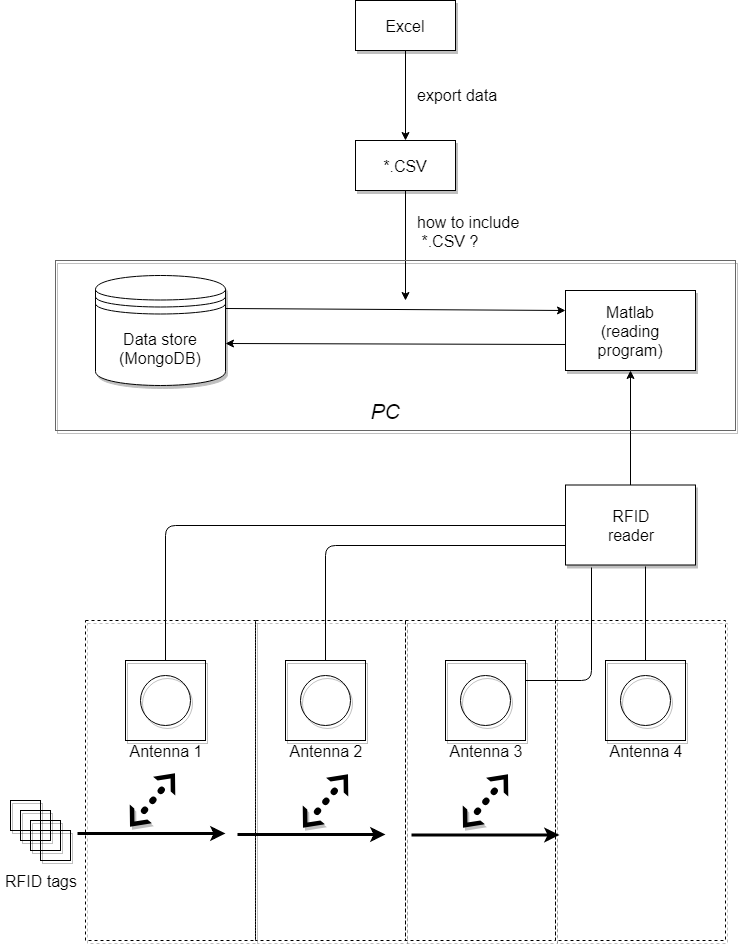
\includegraphics[width=\textwidth]{first_draft} 
\caption{\label{fig:first_draft}The first draft of the developed system} 
\end{figure}

This first concept was changed due to the 'MongoDB' plugin, which offers Matlab \cite{matlab_mongodb}. This is much easier than exporting all received data from Matlab in *.CSV format and then including it into MongoDB as *.CSV data. Furthermore, it supports developing a very fast and real-time application which enables a higher data integrity because of the direct connection to the database (see also figure \ref{fig:app_architecture}.  

%talking about platforms in general, to get a common understanding 
\section{Used platforms and technologies} \label{platforms}

This chapter focusses on explaining the used technologies and frameworks for developping the mobile RFID application. In the following, the framework 'Nativescript' which can be used for native mobile development will be explained. After that, a further section will discuss the technology of NoSQL and will compare it to SQL database technology. This section will also depict MongoDB, a document store. Finally, the Impinj RFID reader will be presented. In the last section \pageref{app_development} of this chapter the challenges as well as the user scenarios will be shown. 

\subsection{Native Development with NativeScript} 

There exist several ways to create a mobile application. But the challenge is to develop a consistent solution for the existing systems, like e.g. Android or iOS.
To face the challenge of developing a hybride solution which can be run both on Android and iOS devices, Nativescript has been established as an open-source project from Telerik in the last years \cite{nativescript}. 

The free and open source technology enables developers to easily build cross-platform native apps with either Javascript, Nativescript or by using Angular \cite{nativescript}. 
Regarding its design philosophy, Nativescript was designed to be approachable to developers from various backgrounds \cite{nativescript}. Moreover, it was designed to be both performant and giving access to native APIs, such as Android or iOS.

Figure \ref{fig:nsarchitecture} gives an impression of the general architecture of Nativescript applications. When developing such applications, one of the given frameworks can be used (e.g. '\{N\} Core', Angular or Vue). Additionally, several Nativescript plugins can be selected. Below the 'NativeScript Core Modules', there are located the 'NativeScript Runtimes' which have direct access to the Native system. By running several commands on the NativeScript \ac{CLI}, the developed Nativescript application can be executed on any physically connected device as well as on the installed emulator or in the cloud. 

\begin{figure}
\centering
\includegraphics[width=\textwidth]{ns-architecture} 
\caption{\label{fig:nsarchitecture}The architecture of NativeScript Applications, adopted from \cite{nsarchitecture}} 
\end{figure}

NativeScript applications can also be developed, built and run on the 'NativeScript Playground' \cite{nsplayground} which enables independent development. Moreover, NativeScript Playground is easier to handle because the development machine does not have to be prepared. Generally, by offering a user-friendly surface, NativSscript Playground is appropriate for beginners who start developing native mobile application.

\paragraph{NativeScript Application Logic}

\begin{figure}
\centering
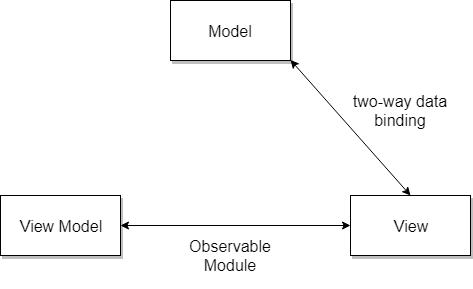
\includegraphics[width=\textwidth]{mvvm_ns} 
\caption{\label{fig:mvvm}The MVVM application logic, adopted from \cite{nativescript}} 
\end{figure}

Nativescript has a \ac{MVVM} application logic (see figure \ref{fig:mvvm}). In contrast to the popular \ac{MVC} application model, Nativescript offers two-way data binding by using the 'Viewmodel' \cite{nativescript}. In every NativeScript application, the model defines and represents data. After that, the data are bound to the view which represents them in a XML file. The 'ViewModel' contains the application logic and exposes all data to the view. 

Between Model and View, data can either be bound as one-way (default setting, the target property updates when a change in the source property occurs) or two-way data binding (all changes in the directions target-source and source-target will be transmitted). To enable the two-way data binding (see figure \ref{fig:mvvm}), the NativeScript Observable Module has to be implemented. 

In the NativeScript Documentation \cite{nativescript} declares the model files as 'Code Behind' because they have the same name as the view file and are written in Javascript or Typescript. By adding attributes to any XML element in the view file, methods can be implemented in the related model file (in Javascript). 

\subsubsection{NativeScript Sidekick} \label{Native}

Nativescript Sidekick is a solution to run the developed application on unsupported platforms in the cloud. It uses both the local build infrastructure and the cloud build service. Nativescript Sidekick offers users to develop with the provided starter templates, to use verified plugins and to build the app in the cloud. Furthermore, Nativescript Sidekick enables developers to debug, test and refactor their application. 
To search for plugins and to manage these, developers can use the Nativescript Marketplace \cite{nsmarket}.

\subsection{NoSQL Technology: MongoDB}\label{mongodb}

As mentioned in section Document Store \pageref{documentstore}, this type of NoSQL database provides high availability, scalability and partitioning options \cite[p.25 ff.]{mongodb_edward}. Nevertheless, there are some disavantages when using MongoDB or any other document stores: For instance, both consistency and transactions are not supported. 

In contrast to relational databases, MongoDB does not consist of tables and rows, but of collections containing documents which make it both flexible and scalable \cite[p.25 ff.]{mongodb_edward}. Collections can be compared to tables in SQL but are schemaless. Instead of having one unique schema within the same collection, every document can have its own set of fields, and common fields can store different values across documents.  

All data is stored in \ac{BSON} documents which assures that related data is placed all together in one place. BSON documents are JSON documents in binary-encoded format. It is the extended form of the JSON data model and is fast, high traversible and lightweight \cite[p.31 ff.]{mongodb_edward}. Moreover, JSON/BSON documents contain schema-less models. Each documents stores data as key-value pairs, where the value can be left blank (see above, disadvantage of consistency). Thus, users of MongoDB have to ensure and check the consistency of their data when adding new data.

One characteristic of MongoDB is the {\_} ID (key) which can be compared to the label or name of a colum in RDBMS. If not explicitely specified by the user, a unique value is automatically generated and assigned  to it by MongoDB. Basically, the key value is immutable and can be of any data type except arrays \cite[p.31 ff.]{mongodb_edward}.

Queries in a MongoDB database use the keys ({\_} ID) in documents which makes it possible to query documents spread across multiple servers. 
MongoDB uses primary-secondary replication, where the primary replication accepts the write requests. To be more precisely, if the write performance needs to be improved, the mechanism of sharding can be used. 

Sharding means that data will be split across multiple machines which are enabled to update different parts of datasets \cite[p.25 ff.]{mongodb_edward}. Besides, this mechanism is automatic in MongoDB, so that as more machines are added, the data is distributed automatically.

\subsubsection{Limitations and possibilities of MongoDB}

There are many advantages and disadvantages, limitatiions and possibilities when using MongoDB. The following paragraph will discuss these and give some examples.

Generally, MongoDB offers many features which MySQL does not. To give an example, MongoDB supports secondary indexes, atomic updates at a per document level. Additionally, queries can be executed by using query documents. Furthermore, MongoDB provides replica sets which are based on master-slave replication with automated failover. After that, MongoDB provides a built-in horizontal scaling. Finally, MongoDB can be run everywhere (e.g. on Cloud, \ac{VM}, servers etc.) because it is written in C++. 

Another feature of MongoDB are 'Capped Collections' which store documents in the inserted order. When the capped collection reaches its storage limit, documents will be deleted from the collection in the inserted order (analogous to \ac{FIFO} principle). Capped collections are often used for log files in order to get these automatically truncated after a certain size. In the end, capped collections guarantee preservation order data in the insertion order \cite[p.31 ff.]{mongodb_edward}.

On the other hand, in contrast to relational databases like MySQL, MongoDB does neither support JOINs nor fully generalized transactions \cite[p.25 ff.]{mongodb_edward}. Secondly, when using MMAPv1 as storage engine, the used space is too large because its data directory files are larger than the database's actual data \cite[p.226 ff.]{mongodb_edward}. For that reason, it is recommended to use MongoDB's WiredTiger storage engine which compresses all files and reduces the storage size by 50\%. Moreover, once a collection is dropped diskspace is automatically reclaimed (unlike MMAPv1 engine).

Thirdly, when using MongoDB BSON documents, their usage is limited the size, nested depth and field limits of the specific document \cite[p.228 ff.]{mongodb_edward}. After that, namespaces as well as indexes are limited, for instance the maximum size of indexed items has to be1024 bytes. The number of indexes per collection must not exceed 64 indexes. Moreover, the usage of sharding is limited \cite[p.230 ff.]{mongodb_edward}. Therefore, if shards were implemented too late, a slowdown of servers is caused because splitting and migration of chunks takes time and resources. Thus, Edward and Sabharwal  recommend to shard a collection before reaching 256 \ac{GB}. 

Next, when using MongoDB, there exist some security limitations because the database does not provide authentication by default. This enables every user which is connected to the database server, to read, change, add and delete data. In addition to that, the connections to and from MongoDB are not encrypted by default. Therefore, when starting the database server on a public network, it is recommended to use encrypted communications. Therefore, Edward and Sabharwal propose the SSL-supported build of MongoDB (which is available as 64-bit version) \cite[p.230 ff.]{mongodb_edward}. 

What is more, using MongoDB implicates write and read limitations, such as case-sensitive queries and type-sensitive fields since there is no enforced schema \cite[p.231 ff.]{mongodb_edward}. For instance, users have to ensure the correctly used type when adding new data. By the same, replica sets which can be used to ensure data redundancy, are limited by the number of the members in every set. When using such replica set, one member acts as a primary member whereas the rest acts like secondary members (a node needs the majority of votes to become primary).

All in all, MongoDB provides many possibilities but also limitations. Generally, it should be clarified that MongoDB is neither adequate to be used in a highly transactional system nor in business intelligence applications where issue-specific databases shall generate highly optimized queries. Finally, it should not be used in applications requiring complex SQL queries. Instead, it is recommended to store high amounts of data and to ensure its availability at any time. 

\subsubsection{MongoDB: Best Practices}

Edward and Sabharwal suggest some 'best practices' when using MongoDB \cite[p.234 ff.]{mongodb_edward} which will be explained briefly in this paragraph. 
First of all, the correct hardware should be chosen. For example, the more internal memory is given, the better the performance of the MongoDB application. Another important point is the CPU: for its productivity, MongoDB needs a fast \ac{CPU} clock speed, as well as a high \ac{RAM}. Moreover, using SATA SSD and \ac{PCI} ensures good price as well as performance results.

Concerning the best practices in coding, Edward and Sabharwal propose to set a correct data model. Further, they recommend avoiding application patterns that lead to unbounded growth of document size as well as to design documents for future which are better to handle with MongoDB's drawback. Besides, documents should be created with an anticipated size where ever applicable. But the most important point when coding is to check data consistency \cite[p.234 ff.]{mongodb_edward}. 

With respect to the data safety and how to provide it in the deployed MongoDB database, Edward and Sabharwal both replication and journaling of data \cite[p.234 ff.]{mongodb_edward}. Furthermore, the repair should be the last resort for recovering data in case of a server crash. Basically, they recommend to always specify a timeout with assuming the command and to run the MongoDB server instance in trusted environment with access control.

Likewise, concerning the administration of MongoDB, Edward and Sabharwal submit to perform instant-in-time backups of durable servers and to use repair in order to compact databases \cite[p.234 ff.]{mongodb_edward}. Correspondingly, managing the replication log is of administrative concern \cite[p.240 ff.]{mongodb_edward}. 

Respecting sharding, it is important to select a good shard key. Moreover, Edward and Sabharwal recommend using three config servers in production deployments to provide redundancy \cite[p.240 ff.]{mongodb_edward}. 

Finally, Edward and Sabharwal introduce 'monitoring' which means that every MongoDB system should be proactively monitored to detect unusual behaviours \cite[p.240 ff.]{mongodb_edward}. To put this into practice, MongoDB's free hosted monitoring service, MongoDB Cloud Manager (which contains a dashboard view of the entire cluster metrics, can be used. Besides, MongoDB itself provides 'mongostat' and 'mongotop' to gain insight into the performance of the database instance (e.g. operation counters, active working sets etc. are shown). 

\subsection{Impinj RFID Lector and Antenna}

The developed system was tested and run on a Speedway R420 RAIN RFID READER \cite{speedway} with four antenna ports (extendable to 32 antennas with an Impinj Antenna Hub \cite{speedway}) and a flexible read range (short and long-range reads are supported). According to the manufacturer's web page \cite{speedway}, the Speedway R420 RAIN RFID READER can be connected to Impinj Autopilot technology which automatically optimizes the reader's operation for its environment. Furthermore, there can be downloaded the appropriate software from the Impinj web page \cite{speedway}.
In the following section, there will be given some information about Impinj, RAIN RFID as well as some example use cases. 

\subsubsection{General Information}

To start with, RAIN RFID will be presented. RAIN RFID is a global alliance promoting universoal adoption of UHF RFID technology \cite{rainrfid}. It can be compared to NFC Forum, WiFi Alliance or Bluetooth SIG. Moreover, RAIN RFID uses a GS1 UHF Gen2 Protocol which is ISO-standardized (18000-63). According to the alliance, the term RAIN shall represent the node between UHF RFID and the cloud where RFID-based data can be stored, managed and shared. Several RAIN RFID uses reader to read and write a tagged item, manage data and take action.

Impinj (also known as NASDAQ:PI) enables wireless connection of multiple everyday items, such as apparel, medical supplies, automobile parts, luggage etc. The Impinj platform uses RAIN RFID to deliver timely information about all items to the digital world (application systems) \cite{impinj}.

\subsubsection{Examples}

Impinj mentions some example use cases when implementing the Speedway R420 RAIN RFID READER: Inventory Management, Asset Tracking and enhanced shopper experience. 
The DeRoyal Industries, Inc. which was founded 1973 is a medical device facturer\cite{deroyal}. With the aim of improving clinical quality and economic health of customers, DeRoyal provides surgical devices, unitized delivery systems, orthopedic supports and bracing wound care dressings.

One of their software solutions is the system 'DeRoyal Continuum Safe' \cite{deroyal}. By using the Impinj platform and RAIN RFID, DeRoyal Continuum Safe automatically captures and tracks data from medical supplies in the operating room, emergency department and catherterization lab. The solution includes packaging which is tagged with RAIN RFID tags. According to DeRoyal, the system provides many advantages, such as reducing the time staff spend managing supplies so that they can focus more on patient care. 

Besides, DeRoyal Continuum Safe improves billing accuracy for supplies used during procedures. After that, the likelihood of infections is reduced by ensuring the availability of necessary supplies. Lastly, DeRoyal achieved to provide a data-driven supply chain management \cite{deroyal}. 

\subsection{Matlab}

According to Dr. Knuth's 'Art of Computer Programming', Matlab is an interpreted language, usually used without an compilation step \cite[lesson 1]{introduction_matlab}. Actually, the Matlab code is converted into machine code by an interpreter as the program is executed. Together with Java, Matlab counts to the high-level languages which on the one hand enables a faster code development but on the other hand limits the speed of execution. Matlab provides a large number of functions for common complicated operations in scientific computing (including engineering and analysis) and technical calculation.

Matlab provides important terminology, like e.g. variables (which contain three fundamental types: characters, real numbers, complex numbers), arguments, commands, command line, scripts, functions as well as comment \cite[lesson 1]{introduction_matlab}. 
One of the most common features of Matlab is its 'Debugger' \cite[lesson 8]{introduction_matlab} which is very usefull for detecting unobvious errors.

Simulink is an add-on product to Matlab which enables an interactive, graphical environment for modeling, simulating, analyzing of dynamic systems \cite[p.313 ff.]{simulink}. Further, it enables rapid constructions of virtual prototypes to explore design concepts at any level of detail with minimal effort \cite[p.313 ff.]{simulink}. For modeling, Simulink provides a GUI for building models as block diagrams so that users are able to produce a 'up-and-running' model. Finally, Simulink is integrated with Matlab and data can be easily shared between the programs.

\subsubsection{Mathworks}

Mathworks is the leader of software development of mathematic calculation, especially for engineers and scientists \cite{mathworks}. Found in 1984, Mathworks is employing more than 3500 employees in 15 countries. Mathworks' headquarters is Natick, Massachusetts, U.S. All Mathworks products are used in various sectors, e.g. automation, airspace, communication, electronics, industrial automization etc. Its main purposes are modeling and simulation which are realized through Matlab and Simulink.

\section{Application development} \label{app_development}

\subsection{Progress of development}

\subsubsection{Challenges during development} \label{challenge}

During the development, many difficulties and challenges had been faced. The following section will focuss on some big problems during development.
To start with, the setup of the development environment of a NativeScript application was complicate because for example on Windows computers there cannot be installed XCode. So, the only solution to develop and run the application both on Android and iOS devices was to use a MacOS computer or to execute the application on Nativescript Sidekick (using its cloud service). Furthermore, during the setup of Android Studio and the runtime environment of Android on MacOS caused other complications. To give an example, sometimes having installed the Android \ac{SDK} 25 the Android \ac{AVD} Manager required exactly the same version being installed on its virtual device. 

Another challenge was the real-time synchronization of the mobile application with MongoDB server was difficult. Firstly, a HTTP request/response was implemented to connect the mobile device with the RFID reader and the database. But using the HTTP request/response was a very static and non-scalable solution (only one device was enabled to connect to the server). Furthermore, refreshing the page was not automated. Thus, another solution had to be considered. Finally, a Socket.IO connection was implemented between both server and client. Socket.IO enables automatic two-way data synchronization and cannot be compared to HTTP Request/Response. By opening a Socket connection between the server and all clients, it was possible to run the application on various mobile devices without any complication. 
After that, another complication was the connection between MongoDB, Matlab and the NativeScript application. This was solved by using a server instance which both connects the database as well as the Nativescript application. Section \ref{section_architecture} explains the exact implementation and the used architecture to connect all system components. 

\subsubsection{User Scenario}

Figure \ref{fig:appfunctionality} gives an example of one user scenario. The figure shows two treatment rooms in a hospital, both equipped with a RFID antenna. In the hallway, there are two additional antennas applied which are connected to the RFID reader. When passing one room, the nurse or doctor will roll a trolley with the needed drugs (all marked with a RFID tag). If the trolley is near to the RFID antenna \#4, it will send the current drug information to the RFID reader which synchronizes them with the computer and the tablet or smartphone. When entering a treatment room, RFID antenna \#3 or \#2 receive the tag's information and synchronize them similarly as before.

At the bottom of the figure, there is a drawn a intranet/internet connection. This means, that the system can be both set up in the local intranet (which enables a higher privacy and security) as well as in the internet. In the end, each RFID antenna can signify a different action, e.g. antenna \#4 = 'medication will be administered', antenna \#3 and \#2 = 'medication is dosed to patient X', \#1 = 'medication has been dosed successfully'.

\begin{figure}
\centering
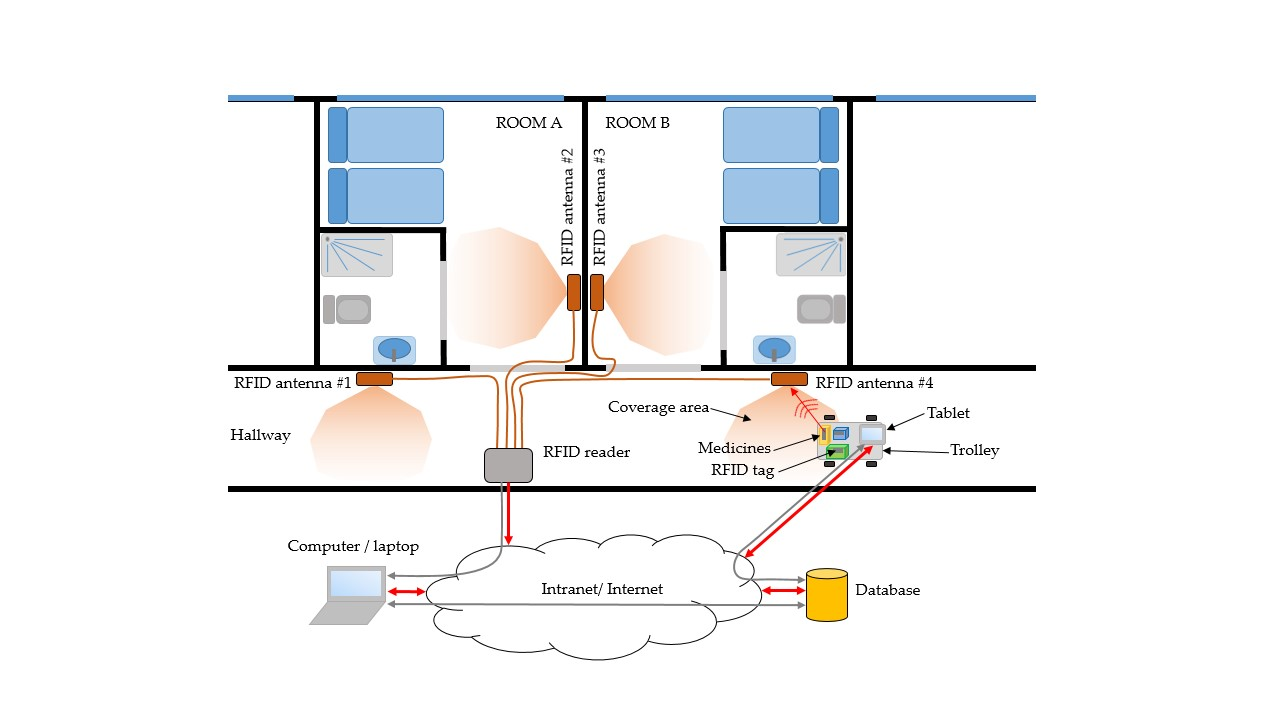
\includegraphics[width=\textwidth]{app_functionality} 
\caption{\label{fig:appfunctionality}Application scenario of RFID application} 
\end{figure}

Figure \ref{fig:app_screenshot} shows two screenshots of both the start and the item information page of the developed application. The photo on the left shows a list of all drugs which are stored in the database. The red point on the right of each data entry signifies that the drug is not available and was not detected successfully. When detecting the specific drug, the colour of the point changes to green.

The picture on the right gives further information of the selected item. Each drug is stored with an 'ID' (which is the same as the RFID tag number). The 'Countrycode' attribute refers to the country-specific number of each drug. For example, in Germany 'Aspirin' has a specific unique code which is called \ac{PZN}, and contains a 7- or 8-place number (e.g. 04114918). The 'Location' attribute describes the exact location of a drug and refers to the location system in the stock (e.g. in pharmacies). The information, 'Timestamp' refers to the last time a drug was detected. The value on the right side of 'Timestamp' is the default value for storing timestamps in MongoDB. If another date format is required, this can be easily defined in the MongoDB schema definition.

\begin{figure}
\centering
\subfigure[Start page of application]{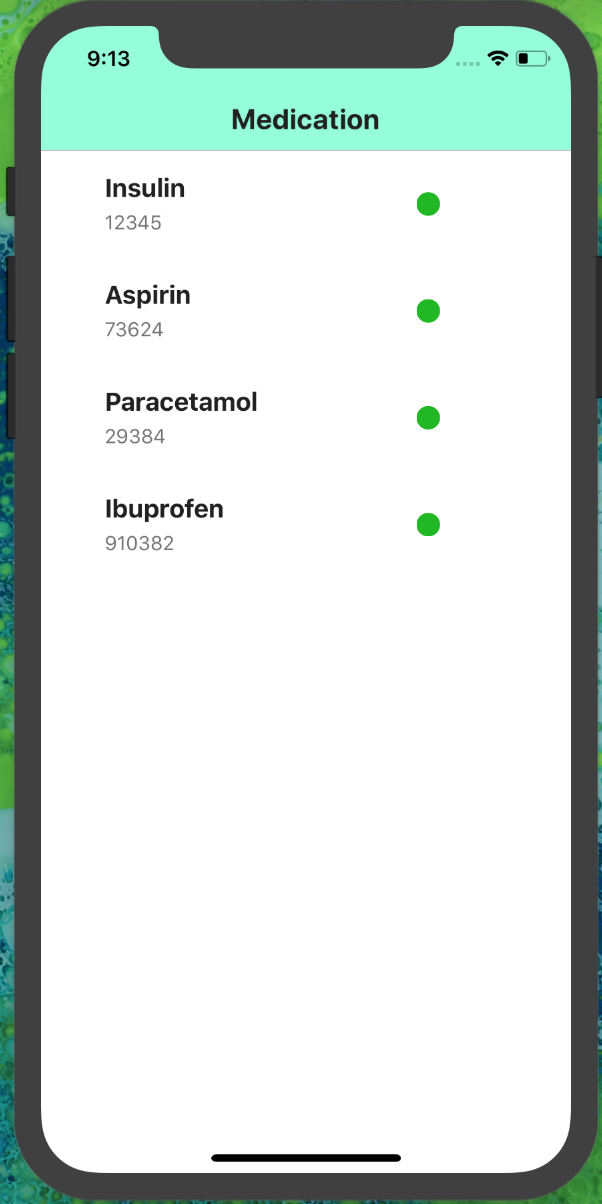
\includegraphics[width=6cm, height=12cm]{Mainview}}
\subfigure[Item information page]{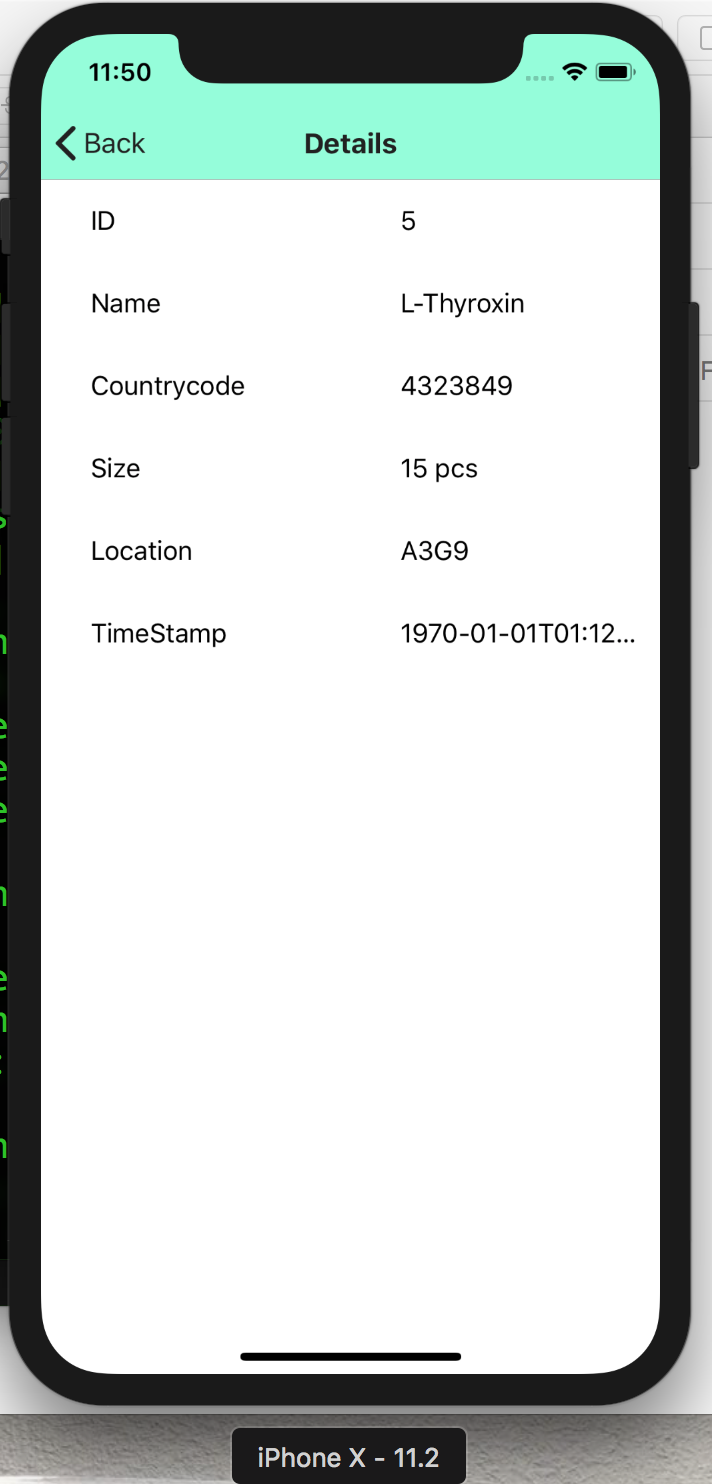
\includegraphics[width=6cm, height=12cm]{Detailview}}
\caption{\label{fig:app_screenshot}Layout of application, Screenshot of iOS Simulator}
\end{figure}

\subsection{Software Architecture} \label{section_architecture}

The following section focusses on the system's architecture which can be seen on figure \ref{fig:apparchitecture}. In the top right corner, there are displayed drugs and patients which can be tagged with a RFID tag. When approximating an antenna of an RFID reader, information about medication (e.g. stock availability ect.) are transmitted. At the same time, the RFID reader registers the detected tag and captures its information using Matlab. Matlab synchronizes the transmitted information with the MongoDB database. When receiving new drug information, the server instance sends the data through a Socket.IO connection to the client (smartphone or tablet). Synchronously, all data is transmitted and displayed on the mobile device.

\begin{figure}
\centering
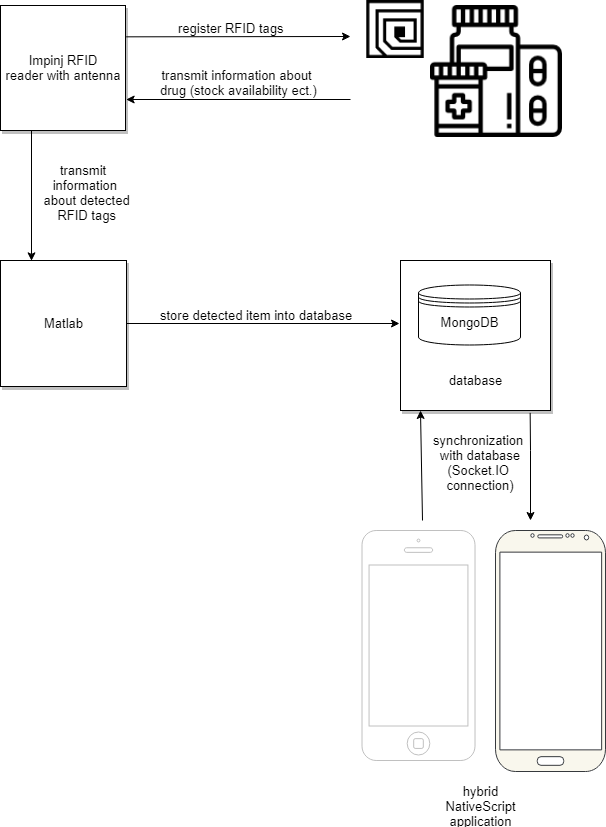
\includegraphics[width=\textwidth]{app_architecture} 
\caption{\label{fig:apparchitecture}The developed system architecture of the mobile RFID application} 
\end{figure}

\subsubsection{Datamodel}

Concerning a useful datamodel, the following figure \ref{fig:datamodel} reflects the outline of the developed MongoDB document related to its context and the MongoDB database. As described in figure \ref{fig:app_screenshot}, 'Details', each drug entry contains information about its ID, name, countrycode, size, location and timestamp. All documents are pooled in a drugs collection which forms a part of medication database. This data model can be extended for example, with other collections, containing information about several equipment or patients. 

\begin{figure}
\centering
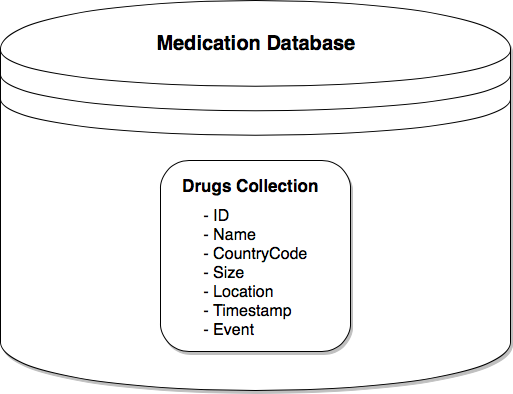
\includegraphics[width=8cm, height=6cm]{Mongo_DataModel} 
\caption{\label{fig:datamodel}Applied data model} 
\end{figure}

\subsubsection{\ac{LAN} Architecture}

Figure \ref{fig:hub_architecture} represents the realization of connecting all relevant components into one LAN. There exist two networks: On the one hand, the LAN between RFID reader, laptop and desktop PC. On the other hand, a local network between the laptop and various mobile devices, like smartphones or tablets is established. The only connecting point between both networks is the laptop with the IP 169.254.1.2.

At the top of figure \ref{fig:hub_architecture}, there is a '5-Port-Ethernet-Hub' which enables connecting up to five different devices or computers via ethernet. 
On the left of the picture, there can be depicted the RFID reader which has the default IP of 169.254.1.1. Each time, when detecting a RFID tag, the RFID reader sends the information to Matlab which is running on the desktop PC with the IP 169.254.1.3. 

After receiving the detected RFID tag's information, the desktop PC transmits the data to MongoDB database running on the laptop with the IP 169.254.1.2. 
The purpose of the second local network between laptop and mobile devices is to execute the NativeScript app and to visualize currently detected RFID tags in the app.

\begin{figure}
\centering
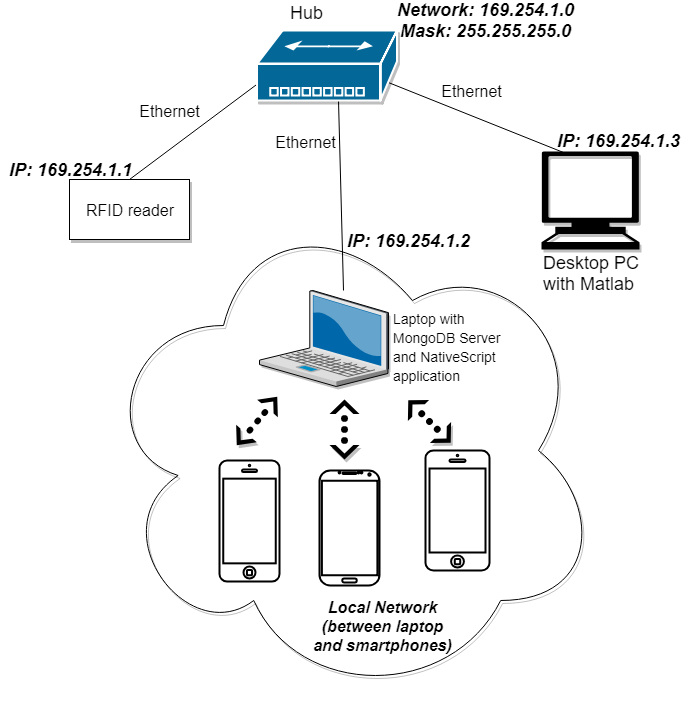
\includegraphics[width=\textwidth]{hub_architecture} 
\caption{\label{fig:hub_architecture}The LAN architecture of the developed system} 
\end{figure}

\subsubsection{Reading Process in Matlab}

The following section focusses on the reading process which is implemented in Matlab. Matlab uses the Impinj Octane SDK \cite{octanesdk} which easily connects the RFID reader to Matlab. The usual reading process in Matlab can be seen in figure \ref{fig:reading_matlab}. In the top left corner of figure \ref{fig:reading_matlab}, after starting the Matlab code, a setup method triggers the initialize method. 

In the time following initializing, Matlab starts reading tags during a predefined time (t). In a loop, every time is read. When reaching the limit of time, the method eventhandlerChanged() is executed. EventhandlerChanged() notices the changes in the detected tags and triggers a new action 'store data'. After that, analogous to the first concept of the system (see section \ref{firstconcept}), the *.mat data is converted into *.csv data and as such exported. In the most current version of the system, the two last actions (conversion and export) are brought together and data is directely transfered into the MongoDB database. 

\begin{figure}
\centering
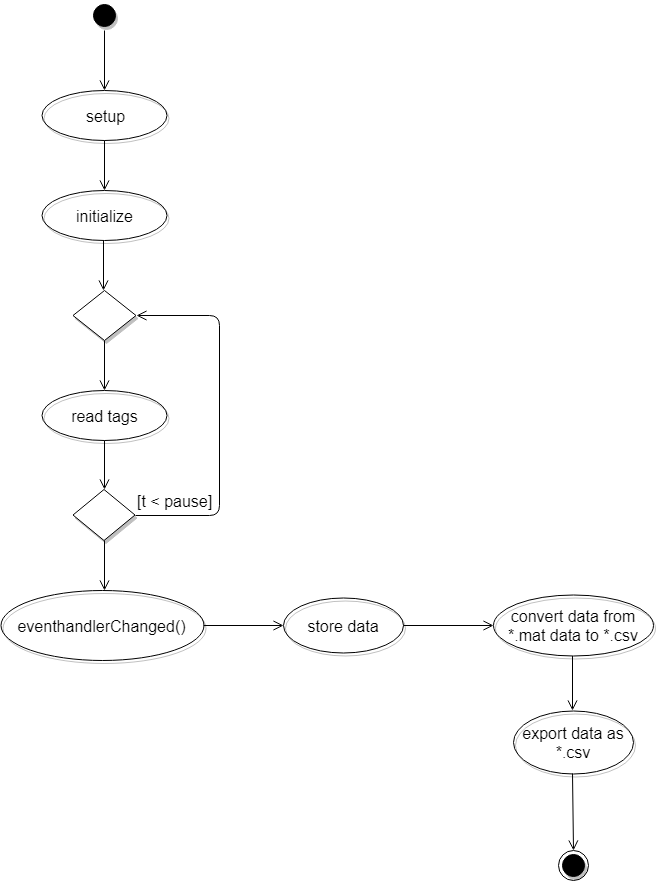
\includegraphics[width=\textwidth]{reading_matlab} 
\caption{\label{fig:reading_matlab}Activity diagram: reading process in Matlab} 
\end{figure}

\section{Tests of system} \label{tests}

\ac{HUCA} which is situated in Oviedo, was created in 13 December 1989 and depends on the 'Servicio de Salud del Principado de Asturias' \cite{huca}. Since 28 February 1990, HUCA has the character of an University Hospital due to the cooperation with the university of Oviedo as well as 'Insalud' and Principado de Asturias, established in 'la Orden'. 
HUCA provides 944 beds, 25 operating suites, 238 rooms for external surgical as well as two gamma cameras (\ac{SPECT}/\ac{TC}) \cite{huca}. Altogether, HUCA is divided into 43 medical subjects, such as Alergology, clinical analysis, clinical biochemistry, surgery, Nephrology, Neurology, Rehabilitation, prevention of work-related risks, radiodiagnostics etc. 

Besides, HUCA forms a part of the 'unit of national reference for work-related illnesses of the respiratory system'. Together with the 'Hospital Monte Naranco', 'hospital del Área Sanitaria IV' and with reference to \ac{SESPA} 'Servicio de Salud del Principado de Asturias' and finally the 'Instituto Nacional de Silicosis', HUCA promotes research on the subject of respiratory disease and its preventions measures.

Figure \ref{fig:permission} shows the permission letter, signed by the director Gloria Herías Correal of HUCA on 8 May 2018 in Oviedo.
The tests are planned for June 2018, an exact date is not fixed already (effective 18 May 2018). 

\begin{figure}
\centering

\includegraphics[width=\textwidth]{permission_HUCA} 
\caption{\label{fig:permission}Permission letter about application tests in HUCA} 
\end{figure}

\subsection{Planned tests of system}

drawing/image of test scenarios...

\subsection{Test results}

\subsection{Evaluation of test results}

\section{Summary and Outlook of application}

which are the problems when employing the system? 
costs of RFID, size of RFID...

\subsubsection{Extension possibilities}

Henrici \cite[p.121 ff.]{henrici} describes four alternative channels to authenticate and authorized the right tags and to prevent attacks on RFID applications. 
The first possibility of an alternative channel is to use written text to authenticate special operations, for instance on packaging. The master key can be printed on the interior of the product package and is proposed as key recovery mechanism.

Furthermore, optical barcodes can be used together with RFID to ensure identification of items. Especially barcodes attached to each item can be used for general identification of objects. Additionally, RFID tags might be used to assign items of high value.

A third possibility of using side channels is to use optical input, such as photodiodes attached to RFID tags. Each RFID tag can use flashes of light (also called optical channel) to transfer data.   
Lastly, a physical contact channel can also be used alternatively. Compared to smartcards, this methods defends against wireless sabotage or denial of service attacks.
